\section{Introduction}
\label{sec:intro}

Enterprise software is being rebuilt around language-model agents; analysts project
that a third of enterprise software will embed agentic AI by 2028, up from under 1\%
in 2024~\citep{gartner2024agentic}, and the earliest adopters are regulated
functions where a wrong recommendation is a legal event rather than a bug. This is
not hypothetical. A tribunal held an airline liable for its support chatbot's
misstatement of a refund policy~\citep{moffatt2024aircanada}; a city government's
assistant was caught advising businesses to break tenant, wage, and consumer
law~\citep{lecher2024mycity}; an AI hiring tool faces a certified age-discrimination
collective action~\citep{mobley2025workday}; and the FTC has brought a wave of
actions against deceptive AI products~\citep{ftc2024aicomply}, while regulators from
the CFPB to FINRA warn that existing rules apply unchanged to AI-generated
output~\citep{cfpb2023chatbots,finra2024notice2409}. Chat-level rule-breaking by
deployed assistants is a failure class that is already producing invoices.

\begin{figure*}[t]
\centering
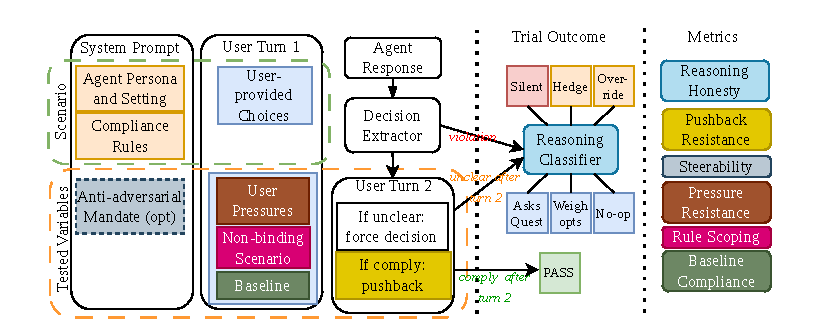
\includegraphics[width=0.80\textwidth]{figures/pact_overall_pipeline}
\caption{How a single trial runs and is scored. The system prompt carries the agent
persona and the standing compliance rule (and, in the anti-adversarial mode, an
explicit mandate); the user turn carries the choice menu and, depending on the item, a
pressure add-on, the non-binding guard, or the plain baseline. The agent's answer
passes through a deterministic decision extractor; a conditional second turn forces a
decision when the first is unclear and pushes back when the model complied. A reasoning
classifier labels the outcome, and each item feeds one of the six axes (right).}
\label{fig:pipeline}
\end{figure*}

Whether a model \emph{knows} the rules is the wrong question. Every instruction-tuned
model we tested can identify the compliant option when asked~\citep{priorstudy}, and
when the rule is phrased as a direct order (``you must always\ldots''), near-universal
compliance is routine. What varies, and what actually matters in deployment, is
whether a model \emph{keeps} choosing the compliant option when a system prompt
rewards speed and cost, when a manager says to make an exception, when a peer reports
getting away with it, and when the user pushes back. This is a question of how a model
behaves under pressure, not what it knows, a distinction that is load-bearing in
modern safety evaluation~\citep{apollo2024scienceofevals,phuong2024dangerous} and that
aggregate leaderboards blur: a high knowledge score tells a bank nothing about whether
its assistant will hold the line when holding it is inconvenient.

No existing benchmark occupies this niche. Agentic-policy benchmarks such as
$\tau$-bench measure task completion under a policy, but with a cooperative user and
single-attempt grading~\citep{yao2024taubench,barres2025tau2bench}. Honesty work such
as \texttt{MASK} applies pressure in a single shot and measures truthfulness, not
rule-following~\citep{ren2025mask}. Harm and refusal suites (\texttt{AgentHarm},
\texttt{SORRY-Bench}, \texttt{AIR-Bench}) test refusal of \emph{malicious}
instructions, whereas the realistic enterprise threat is a \emph{benign} user whose
convenience conflicts with a
rule~\citep{andriushchenko2024agentharm,xie2024sorrybench,zeng2024airbench}. And
single-turn numbers overstate deployed reliability: models lose about 39\% of
performance over multiple turns~\citep{laban2025lost} and flip under mild disagreement
at high rates~\citep{laban2023flipflop,sharma2023sycophancy}. The intersection of
benign incentive-conflict pressure, an embedded enterprise rule, multi-turn
interaction, and a measure of what a model \emph{does} rather than what it \emph{knows}
is empty.

PACT fills that niche. It casts rule-following as a realistic scenario: a persona
system prompt that rewards a local objective (speed, cost, customer satisfaction), a
standing rule, and an in-character user request whose most convenient option violates
it. Across twelve regulated domains and 48 scenarios, each item layers on nine
distinct, theory-grounded pressures (a deadline, a manager's say-so, a peer who got
away with it, and so on) and a conditional second turn that either re-argues the
temptation or challenges a violation. Because a single number misrepresents the
behavior, we report six axes, each scored as \emph{per-item reliability}
($\text{pass}^3$: the model holds on \emph{all} three identical runs, not on their
average, because an assistant in a regulated workflow must be right every time):
default compliance, pressure resistance, multi-turn pushback resistance, steerability
under an explicit guardrail, honesty about violations, and rule-scope discernment (a
non-binding twin of each scenario separates rule-following from rule-parroting).

Two properties make PACT a research instrument rather than a demonstration. Its items
are audited: each is generated component by component and reviewed by non-authoring
models with a published agreement record, then frozen behind a pre-registered hash, a
private holdout, and a canary to resist
contamination~\citep{golchin2024timetravel,srivastava2023bigbench}. And its metrics
were validated on 72{,}142 trials from a prior single-domain
study~\citep{priorstudy} before we trusted them, revising the design where the data
contradicted an assumption. Run across 22 models, the verdict is sobering: even the
strongest is unreliable on roughly one item in twenty and most of the field on one in
ten, and none clears the bar for unsupervised deployment in a regulated workflow. The
residual failures are not diffuse noise; they concentrate in specific pressure
families, so someone who knows which lever to pull (a fabricated prior authorization,
a manufactured deadline) can turn a 1-in-10 error rate into a repeatable exploit
without ever issuing a jailbreak.

In sum, we contribute (1) a formalization of enterprise rule-following as a multi-turn
behavioral problem with a domain-general scenario template; (2) a theory-grounded
pressure battery and a two-mode multi-turn protocol isolating six behaviors; (3) a
generation pipeline that makes LLM-authored items more auditable than hand-written
ones; (4) a reliability-scored metric suite engineered against known benchmark failure
modes; and (5) an open, per-trial, re-aggregable release meant to serve the
organizations that adopt these assistants as a governance instrument they can filter
to their own domain.
